\documentclass[../Head/Main.tex]{subfiles}
\begin{document}

\subsection{Lidar Scanner}
The two-wheeled robot given for this project is among other equipped with a 2d lidar (Light Detecting and Ranging) scanner. A lidar scanner detects the distance to targets by emitting a laser pulse and analyzing the time it takes for the beam to reflect and return to its source. The lidar scanner maps the environment and has a detecting range of 10 pixels in Gazebo and a 260 degrees field of view. \par
The script converts this range into mm by first scaling the pixel map to double size, such that the detecting range is 20 pixels. Afterwards, the script trace the pixel map to a eps-figure using 72 dpi as standard 
for the postscript. Then, the script converts this range from inches to mm by using a conversion factor of 25.4 mm per inch. This means that this range can be converted into mm by using the following formula:
\begin{align*}
\frac{20~pixels}{72~dpi}\cdot 25.4~\frac{mm}{inch} = 7.06~mm
\end{align*}
Now the script scales the world from mm to m, which means that the range of the lidar scanner therefore is 7.06 m.\par
The lidar scanner maps the surrounding environment by collecting 200 datapoint, which must be processed in order to recognize objects such as walls and marbles. This means that circle and line detecting algorithms must be writing. \par
The datapoints from the lidar scanner is first visualized by drawing white lines from the robot’s location to each of the 200 datapoints using the \texttt{cv::line()} function as shown on figure \ref{fig:white_lines}. Afterwards the datapoints are sorted by checking if the range is equal to max detecting range in order to get the points, that reflects from different object.\par
The rest of the datapoints are drawn as lines upon the unsorted data. These lines can be distinguished by different blue colours depending on the range between the two points ranging from blue to cyan. This blue coloured and white lines are shown on figure \ref{fig:blue_lines}.

\begin{figure}[H]
  \begin{subfigure}[b]{0.49\textwidth}
    \centering
    
\includegraphics[width=0.5\textwidth]{lidar_test_Two_v1}
    \caption{Illustration of the unsorted data}
    \label{fig:white_lines}
  \end{subfigure}
  \hfill
  \begin{subfigure}[b]{0.49\textwidth}
  	\centering
    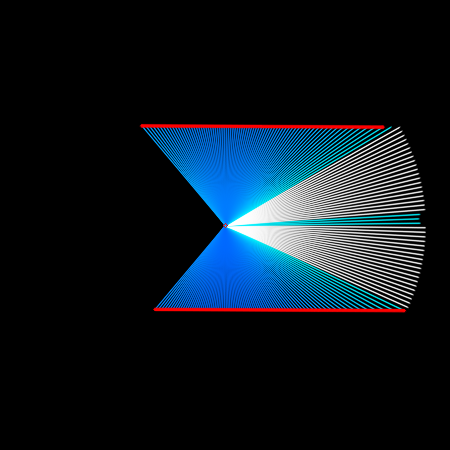
\includegraphics[width=0.5\textwidth]{lidar_test_Two_v2}
    \caption{Illustration of the soted data}
    \label{fig:blue_lines}
  \end{subfigure}
  \caption{Illustration of the sorted and unsorted data}
\end{figure}
\subfile{../Sections/Design_line_detection}
\subfile{../Sections/Design_marble_detection}

\end{document}